\documentclass[oneside, 12pt]{book}
\usepackage{icdthesisUTF}
\usepackage{tabularx} 
\usepackage{epsfig}
\usepackage{listings}
\usepackage{xcolor}
\lstdefinestyle{sharpc}{language=[Sharp]C, rulecolor=\color{blue!80!black}}

\renewcommand{\thesistitle}{Ανάπτυξη eργαλείου για την σχεδίαση παιχνιδιών με την βοήθεια υπο-λογιστή }
\renewcommand{\thesisauthor}{Γιώργου Μιχαηλίδη}
\renewcommand{\thesisauthorabbrv}{Γ. Μιχαηλίδης}
\renewcommand{\thesisauthorinitials}{ΓΜ}
\renewcommand{\thesissupervisor}{Δρ. Νικόλαος Πεταλίδης. Επιστημονικός Συνεργάτης}
\renewcommand{\thesismonth}{Φεβρουάριος}
\renewcommand{\thesisyear}{2016}

% Η βιβλιογραφία
\addbibresource{testUTF.bib}

\begin{document}
	
	\Titlepage
	\Declarationpage
	
	\begin{Abstract}
		Τα πρώτα ηλεκτρονικά παιχνίδια είχαν γραφτεί εξ'ολοκλήρου σε υλισμικό. Από τότε, οι κάρτες γραφικών και οι μικροεπεξεργαστές βελτιώθηκαν, δημιουργήθηκαν κονσόλες φτιαγμένες αποκλειστικά για ηλεκτρονικά παιχνίδια, με ειδικά χειριστήρια τα οποία σου προσφέρουν διαφορετικές εμπειρίες.
		Η διαδικασία ανάπτυξης λογισμικού είναι ακριβή και ο σχεδιασμός γίνεται όλο πιο σύνθετος και περίπλοκος. Τα έργα γίνονται όλο πιο απαιτητικά και δαπανηρά. Δημιουργήθηκε η ανάγκη για ένα εργαλείο το οποίο να παρέχει ένα ομοιογενές περιβάλλον για την ανάπτυξη σύνθετων έργων. 
		Ένα CASE (Computer Aided Software Engineering) tool είναι ένα λογισμικό-εργαλείο το οποίο απλοποιεί τον κύκλο ανάπτυξης ενός λογισμικού. 
		Στο τομέα του σχεδιασμού παιχνιδιών το πιο διαδεδομένο CASE tool είναι η μηχανή γραφικών. Μια μηχανή γραφικών είναι μια σουίτα από επαναχρησιμοποιήσιμα οπτικά εργαλεία τα οποία βρίσκονται σε ένα ενιαίο περιβάλλον.
		Σκοπός της πτυχιακής είναι να αναγνωριστούν μοτίβα και τεχνικές δημιουργίας παιχνιδιών, ώστε να δημιουργηθεί ένα εργαλείο το οποίο να το προσεγγίζει από υψηλό επίπεδο με αφαιρέσεις για εύκολη μοντελοποίηση και αυτοματοποίηση κατά τη δημιουργία.
	\end{Abstract}
	\tableofcontents
	\listoftables
	\listoffigures
	
	\begin{Preface}
	\paragraph{Σκοπός} 
	Σκοπός της πτυχιακής είναι να εξηγήσει θεωρητικά και πρακτικά τα κομμάτια που απαρτίζουν μια
	τυπική μηχανή γραφικών και πώς συνδέονται αρχιτεκτονικά μεταξύ τους, μαζί με παραδείγματα και οδηγίες για την επέκτασή τους. Για το κομμάτι του rendering, δεν  έγινε απευθείας με προτόκολο που επικοινωνεί με την κάρτα γραφικών, αλλά με την ανοικτού λογισμικού βιβλιοθήκη monogame η οποία είναι και cross-platform,  δηλαδή ανάλογα με το περιβαλλον ανάπτυξης χρησιμοποιεί το ανάλογο προτόκολο για επικοινωνία με την κάρτα γραφικών, για παράδειγμα για Linux OS χρησιμοποιεί OpenGL και για Android ΟpenGL ES, για να επικεντρωθεί στο rendering γενικά και όχι για συγκεκριμένη πλατφόρμα. Τα παραδείγματα αξιοποιούν object-oriented και functional paradigms και είναι γραμμένα σε C\#.

	\paragraph{Θεμελίωση} 	
	Οι μηχανές γραφικών διαφέρουν με βάση τις λεπτομέριες αρχιτεκτονικής και υλοποίησης, αλλά τα πρότυπα σχεδίασης είναι καθολικά. Πρακτικά, οι μηχανές γραφικών απαρτίζονται από τις ίδιες βασικές έννοιες. Πολλά βιβλία έχουν γραφτεί τα οποία εστιάζουν στην κάθε έννοια ξεχωριστά αλλά ελάχιστα για το πως αυτά τα στοιχεία επικοινωνούν και αλληλεπιδρούν μεταξύ τους. 
	Η εργασία εστιάζει στην αρχιτεκτονική των μηχανών, 
	για το πώς οι ομάδες είναι οργανωμένες για να δουλεύουν μεταξύ τους, 
	ποια συστήματα και μοτίβα επαναλαμβάνονται στη δημιουργία μηχανών, 
	ποιες είναι οι απαιτήσεις για το κάθε μεγάλο υποσύστημα της μηχανής, 
	ποια συστήματα είναι αγνωστικιστικά σε παιχνίδια ή σε είδη παιχνιδιών και ποια είναι συγκεκριμένα,
	και πότε σταματά η μηχανή και ξεκινά η υλοποίηση του παιχνιδιού.
	
	Eπιπρόσθετα, θα γίνει σύγκριση με άλλες δημοφιλείς μηχανές γραφικών και βιβλιοθηκών τεχνικές για configuration management, versioning και διάφορα συστήματα ανάπτυξης. 
	\end{Preface}
	
	\begin{Acknowledgement}
		Ευχαριστίες (στο μπαμπά, στη μαμά, κτλ)
	\end{Acknowledgement}
	
	\begin{Definitions}
		Ορισμοί εννοιών που μπορεί να είναι χρήσιμοι. Για παράδειγμα:	
		\begin{description}
			\item [\LaTeX] Σύστημα στοιχειοθεσίας κειμένων
		\end{description}
		
	\end{Definitions}
	
	\chapter{Εισαγωγή}
			
		\leftmark\rightmark
		\section{Η τυπογραφία σήμερα}
		Αυτή είναι η αναφορά σε ένα άρθρο περιοδικού:\citep{Schmidt98}.Αυτή
		είναι η αναφορά σε ένα βιβλίο:\citep{goosens93}. Αυτή είναι η αναφορά
		σε ένα ελληνικό βιβλίο:\citep{Chatzigeorgiou05}. Βιβλίο στα ελληνικά
		με ξένο συγγραφέα:\citep{Sommerville09}. Άρθρο σε
		συνέδριο~\citep{4343930}. 
		
		Τέλος αναφορά σε ιστοσελίδα:~\citep{Wikipedia_BibTeX}.
		
		Εδώ αναφερόμαστε στo σχήμα~\ref{fig:image1}:
		\begin{figure}[h]
			\centering
			
\includegraphics[width=35mm]{lion.png}
			\caption{Παράδειγμα εικόνας}
			\label{fig:image1}
		\end{figure}
		
		και εδώ στον πίνακα~\ref{tab:table1}:
		\begin{table}[h]
			\centering
			\caption{Παράδειγμα πίνακα}
			\begin{tabularx}{\linewidth}[h]{|XXX|}%
				\hline
				\hline
				Κίνητρα & Παραδείγματα ευρημάτων & Αριθμός μελετών\\
				\hline
				Ταύτιση με το έργο & Ξεκάθαροι στόχοι &20\\
				Καλό management & Ομαδικότητα &16\\
				Συμμετοχή υπαλλήλων & Συμμετοχή στις αποφάσεις&16\\
				Προοπτικές εξέλιξης & Προοπτικές προαγωγής&15\\
				Ποικιλία στην εργασία & Καλή χρήση ικανοτήτων& 14\\
				Αίσθηση του να ανήκεις κάπου& Υποστηρικτικές σχέσεις&14\\
				Αμοιβές και κίνητρα & Αυξημένος μισθός& 14\\
				\hline
				\hline
			\end{tabularx}
			\label{tab:table1}
		\end{table}
		\appendix
	
	\chapter{Case Tools}
	Η διαδικασία ανάπτυξης λογισμικού είναι ακριβή και ο σχεδιασμός γίνεται όλο πιο σύνθετος και περίπλοκος. Τα έργα γίνονται όλο πιο απαιτητικά και δαπανηρά. Δημιουργήθηκε η ανάγκη για ένα εργαλείο τιο οποίο να παρέχει ένα ομοιογενές περιβάλλον για την ανάπτυξη σύνθετων έργων. 
	Ένα CASE (Computer Aided Software Engineering) tool είναι ένα λογισμικό-εργαλείο το οποίο απλοποιεί τον κύκλο ανάπτυξης ενός λογισμικού. Τα Case Tools γίνονται όλο και πιο δημοφιλές, λόγω της βελτίωσης των δυνατοτήτων και της λειτουργικότητας στην ανάπτυξη της ποιότητας του λογισμικού. Η διαδικασία ανάπτυξης αυτοματοποιείται, και συντονίζεται. Το λογισμικό συντηρείται και αναλύεται εύκολα. 
	
	Κάποιες κοινές λειτουργίες τους είναι:
	\begin{itemize}
	\item Δημιουργία ροής δεδομένων και μοντέλων οντοτήτων.
	\item Καθιέρωση της σχέσης μεταξύ απαιτήσεων και προτύπων.
	\item Ανάπτυξη του σχεδιασμού σε υψηλό επίπεδο.
	\item Ανάπτυξη λειτουργικών και διαδικαστικών περιγραφών
	\item Ανάπτυξη περιπτώσεων δοκιμών (test cases).	
	\end{itemize}
	
	Γιατί να χρησιμοποιήσει κάποιος;
	\begin{itemize}
	\item Γρήγορη εγκατάσταση
	\item Εξοικονόμηση χρόνου μειώνοντας τον χρόνο στον προγραμματισμό και στις δοκιμές.
	\item Οπτικοποίηση του κώδικα και της ροής δεδομένων
	\item Βέλτιστη χρήση των διαθέσιμων πόρων.
	\item Ανάλυση, ανάπτυξη και σχεδιασμό με ενιαίες μεθοδολογίες.
	\item Δημιουργία και τροποποίηση τεκμηρίωσης (documentation)
	\item Αποτελεσματική μεταφορά πληροφοριών ανάμεσα στα διάφορα εργαλεία
	\item Γρήγορη δημιουργία λογισμικού.
	\end{itemize}
	
	Πώς να χρησιμοποιηθεί
	\begin{itemize}
	\item Για να διευκολυνθεί η μεθοδολογία σχεδιασμού. 
	\item Για Rapid Application Development
	\item Testing
	\item Documentation
	\item Project Management
	\item Μειωμένο κόστος συντήρησης
	\item Αύξηση της παραγωγικότητας:
	\end{itemize}
	H Αυτοματοποίηση των διαφόρων δραστηριοτήτων των διαδικασιών ανάπτυξης και διαχείρισης του συστήματος αυξάνει την παραγωγικότητα της ομάδας ανάπτυξης.
	
	Χαρακτηριστικά ενός καλού case tool
	\begin{itemize}
	\item Τυποποιημένη μεθοδολογία χρησιμοποιώντας τεχνικές μοντελοποίησης όπως UML.
	\item Flexibility: το εργαλείο πρέπει να προσφέρει τη δυνατότητα στο χρήστη να επιλέγει ποια εργαλεία να χρησιμοποιήσει.
	\item Strong integration: το εργαλείο πρέπει να υποστηρίζει όλα τα στάδια ανάπτυξης. Όταν γίνεται μια αλλαγή, τα στάδια τα οποία επιρεάζονται πρέπει να τροποποιούνται κατάλληλα.
	\item Ενσωμάτωση με εργαλεία ελέγχου.
	\item Reverse-engineering: δυνατότητα δημιουργίας κώδικα από δεδομένα
	\end{itemize}
		
	\chapter{Game Engineering}
			
	\subsection{Μηχανές Γραφικών}
	Στο τομέα του σχεδιασμού παιχνιδιών το πιο διαδεδομένο CASE tool είναι η μηχανή γραφικών. Μια μηχανή γραφικών είναι μια σουίτα από επαναχρησιμοποιήσιμα οπτικά εργαλεία τα οποία βρίσκονται σε ένα ενιαίο περιβάλλον.
	Η κεντρική λειτουργικότητα η οποία παρέχεται περιλαμβάνει τη φωτοαπόδοση σε πραγματκό χρόνο (real time rendering) , τη μηχανή φυσικής και εντοπισμό συγκρούσεων (physics and collision detection), το scripting, το animation, την τεχνητή νοημοσύνη (Artificial Intelligence), τη δικτύωση (networking), τον παραλληλισμό ενεργειών (multitasking), την διαχείριση μνήμης και τον γράφο σκηνής (scene graph). Η ανάπτυξη τον παιχνιδιών μέσω μιας μηχανής γραφικών γίνεται εύκολα, γρήγορα και οδηγούμενη απο δεδομένα (data driven) ούτως ώστε οι δημιουργοί παιχνιδιών να μπορούν να ασχολούνται με τις λεπτομέρειες του παιχνιδιού τους.
	Οι μηχανές αναπτύσσονται από ομάδες που απαρτίζονται όχι μόνο από προγραμματιστές, αλλά και απο μαθηματικούς, φυσικούς κλπ. Η κάθε υπο-ομάδα εστιάζει σε ένα συγκεκριμένο κομμάτι, όπως οι φυσικοί με τον εντοπισμό συγκρούσεων, και αρχιτέκτονες λογισμικού σχεδιάζουν το πως τα κομμάτια συνδέονται και αλληλεπιδρούν μεταξύ τους, χωρίς να τους απασχολούν οι λεπτομέριες σχεδίασης του κάθε κομματιού.
	
	\paragraph{Ιστορία}
	Η ιστορία των Βιντεοπαιχνιδιών, αρχίζει στα τέλη της δεκαετίας του '40. Προς τα τέλη του '50 και στα μέσα του '60, στην Αμερική, αρχίζουν να μπαίνουν στην καθημερινή μας ζωή, οι υπολογιστές. Για την ακρίβεια, οι κεντρικοί υπολογιστές. Από εκείνη την περίοδο, τα βιντεοπαιχνίδια έκαναν την εμφάνιση τους, στις κονσόλες, στα φλίπερ, στους υπολογιστές, αλλά και στις φορητές κονσόλες. Από τότε η δημιουργία παιχνιδιών έχει γιγαντιωθεί έχοντας ένα τεράστιο κομμάτι της παγκόσμιας οικονομίας.
	Πλέον ο ανταγωνισμός είναι τεράστιος, τα βιντεοπαιχνίδια κυκλοφορούν για διάφορες κονσόλες με  πολύ απαιτητικά γραφικά και με πολύ γρήγορο ρυθμό.
	
	\paragraph{Δομή μιας τυπικής ομάδας ανάπτυξης παιχνιδιών}
	Πριν από την ανάλυση της δομής της μηχανής, θα γίνει ανάλυση της δομής ομάδας η οποία θα την χρησιμοποιεί για να αναπτυχθούν στοχευμένα εργαλεία για το κάθε πρόβλημα της κάθε υποομάδας.
	
	\paragraph{Μηχανικοί}	
	Οι μηχανικοί σχεδιάζουν και υλοποιούν το λογισμικό του παιχνιδιού και τα εργαλεία τα οποία χρησιμοποιούνται για την ανάπτυξή του. Οι δύο μεγάλες κατηγορίες μηχανικών είναι οι
	\begin{itemize}
		\item runtime programmers οι οποίοι ασχολούνται με τη μηχανή κται το παιχνίδι 
		\item tool programmers οι οποίοι γράφουν tools τα οποία αυτοματοποιούν και ευκολύνουν την διαδικασία ανάπτυξης.
	\end{itemize}
	Οι μηχανικοί έχουν είτε κάποια ειδικότητα, για παράδειγμα ειδικότητα στη τεχνητή νοημοσύνη, είναι είναι generalists, δηλαδή κατέχουν από όλα τα στοιχεία και μπορούν να λύσουν προβλήματα που κατά τη διάρκεια ανάπτυξης.
	
	\paragraph{Artists}
	Οι artists παράγουν όλο το οπτικοακουστικό κομμάτι του παιχνιδιού, το οποίο είναι βασικό κομμάτι για το χαρακτήρα του παιχνιδιού. Χωρίζονται στις εξής κατηγορίες
	
	\begin{itemize}
		\item Concept artists οι οποίοι σχεδιάζουν σκίτσα και πίνακες τα οποία παρέχουν στην ομάδα την εικόνα του τελικού παιχνιδιού. Παρέχουν οπτική καθοδήγηση στην ομάδα καθ' όλη τη διάρκει του κύκλου ανάπτυξης.
		\item 3D Modelers οι οποίοι είναι υπεύθυνοι για την τρισδιάστατη γεωμετρία του εικονικού κόσμου του παιχνιδιού. Απαρτίζονται από τους
		foreground modelers οι οποίοι σχεδιάζουν χαρακτήρες, οχήματα, οπλα και αντικείμενα του τρισδιάστατου κόσμου
		background modelers οι οποίοι σχεδιάζουν την στατικό περιβάλλον πχ κτήρια
		\item Texture artists οι οποίοι σχεδιάζουν τις δισδιάστατες εικόνες που καλύπτουν τα τρισδιάστατα μοντέλα
		\item Lighting artists που ορίζουν τις στατικές και δυναμικές πηγές φωτός και δουλεύουν με το χρώμα, την κατεύθυνση και την κατεύθυνση του φωτός.
		\item Animators οι οποίοι σχεδιάζουν την κίνηση των χαρακτήρων και των αντικειμένων
		\item Motion capture actors οι οποίοι παρέχουν ακατέργαστα δεδομένα κίνησης για να επεξεργαστούν οι animators και να τα ενσωματώσουν στο παιχνίδι.
		\item Sound designers οι οποίοι παράγουν τα εφέ και τη μουσική.
		\item Voice actors τους οποίους η φωνή ηχογραφείται και χρησιμοποιείται για τους χαρακτήρες στο παιχνίδι
	\end{itemize}
	
	\paragraph{Game Designers}
	Η δουλειά ενός game designer είναι να σχεδιάσει το διαδραστικό τμήμα του παιχνιδιού, το gameplay. Ασχολούνται με τον σχεδιασμό επιπέδων, την ιστορία τηις αλληλεπιδράσεις μεταξύ των χαρακτήρων στο παιχνίδι με τους στόχους, σκοπούς και κανόνες του παιχνιδιού.
	Σχεδιάζουν το κάθε επίπεδο μονδικά και αποφασίζουν για τη γεωμετρία στο περιβάλλον, πότε και που εμφανίζονται χαρακτήρες και διάφορα αντικείμενα, πως γίνονται οι μεταβάσεις μεταξύ διάφορων σκηνών κλπ.
	
	\paragraph{Producers}
	Ο ρόλος του producer διαφέρει από στούντιο σε στούντιο. Η βασική του δουλειά είναι να προγραμματίζει και να δρομολογεί τις διάφορες εργασίες και να λειτουργεί ως ο συνδετικός κρίκος μεταξύ των ατόμων που παίρνουν ηγετικές αποφάσεις και την ομάδα ανάπτυξης. Οι producers είναι χαρακτηριστικό των ΑΑΑ εταιριών, όπου υπάρχουν πολλά τμήματα και πολλοί εργαζόμενοι.
		
	\paragraph {Τι είναι μια μηχανή γραφικών}
	Η πρώτη αναφορά ε μηχανή γραφικών έγινε στα μέσα της δεκαετίας του 90 και αναφερώταν στο δημοφιλές παιχνίδι Doom του οποίου η αρχιτεκτονική διαχώριζε τα βασικά συστήματα του παιχνιδιού, όπως rendering system, collision detection system, audio system, asset system κλπ. Η αξία αυτού του διαχωρισμού εκτιμήθηκε από την κοινότητα όταν οι προγραμματιστές ξεκίνησαν να πουλάνε άδειες για το λογισμικό, επαναχρησιμοποιούσαν εργαλεία προηγούμενων παιχνιδιών με δημιουργία νέων assets. Μικρότερα στούντιο τροποποιούσαν εκδόσεις υπάρχων παιχνιδιών χρησιμοποιωντας το SDK.ό
	Πολλά παιχνίδια γράφτηκαν με σκοπό να επαναχρησιμοποιηθούν κομμάτια κόδικα και modding. Πολλές μηχανές όπως η μηχανή του Quake III γράφτηκαν με τρόπο ώστε να είναι εύκολα προσαρμόσημες χρησιμοποιώντας scripting, με σκοπό την εμπορευματοποίηση μέσω licensing.
	Η διαχωριστική γραμμή μεταξύ του παιχνιδιού και της μηχανής δεν μπορεί να οριστεί με ακρίβεια. Πολλές μηχανές μπορεί να περιέχουν συγκεκριμένα μέρη που αφορούν συγκεκριμένη λειτουργία του παιχνιδιού. Η μεγάλη διαφορά είναι στο data-driven architecture όπου οι κανόνες και τα στοιχεία δεν είναι hard-coded αλλά διαβάζονται από εξωτερικό αρχείο.
	Οι μηχανές έχουν τα όριά τους ανάλογα με τα είδη παιχνιδιού στα οποία η μηχανή εστιάζει, σε ποιες πλατφόρμες, σε τι στιλ γραφικών, σε ποια αρχιτεκτονική της gpu κλπ. 
	
	\paragraph{Γιατί μηχανές γραφικών;}
	
	Η αφαίρεση πάντα βοηθούσε τον εγκέφαλο να λειτουργήσει καλύτερα και να κατανοήσει αλληλεπιδράσεις μεταξύ συστημάτων και περίπλοκες έννοιες. Οι μηχανές γραφικών απαλλάζουν τους γραφίστες και τους προγραμματιστές από τις τεχνικές λεπτομέριες, και εστιάζουν στην αισθητική και στο gameplay. Επίσης με την αποσύνδεση των συστημάτων έχουμε πιο προβλέψημη συμπεριφορά, επεκταστημότητα των υποσυστημάτων ως υποσυστήματα και ευκολη δοκιμαστικότητα.
	
	\begin{figure}[h]
		\centering
		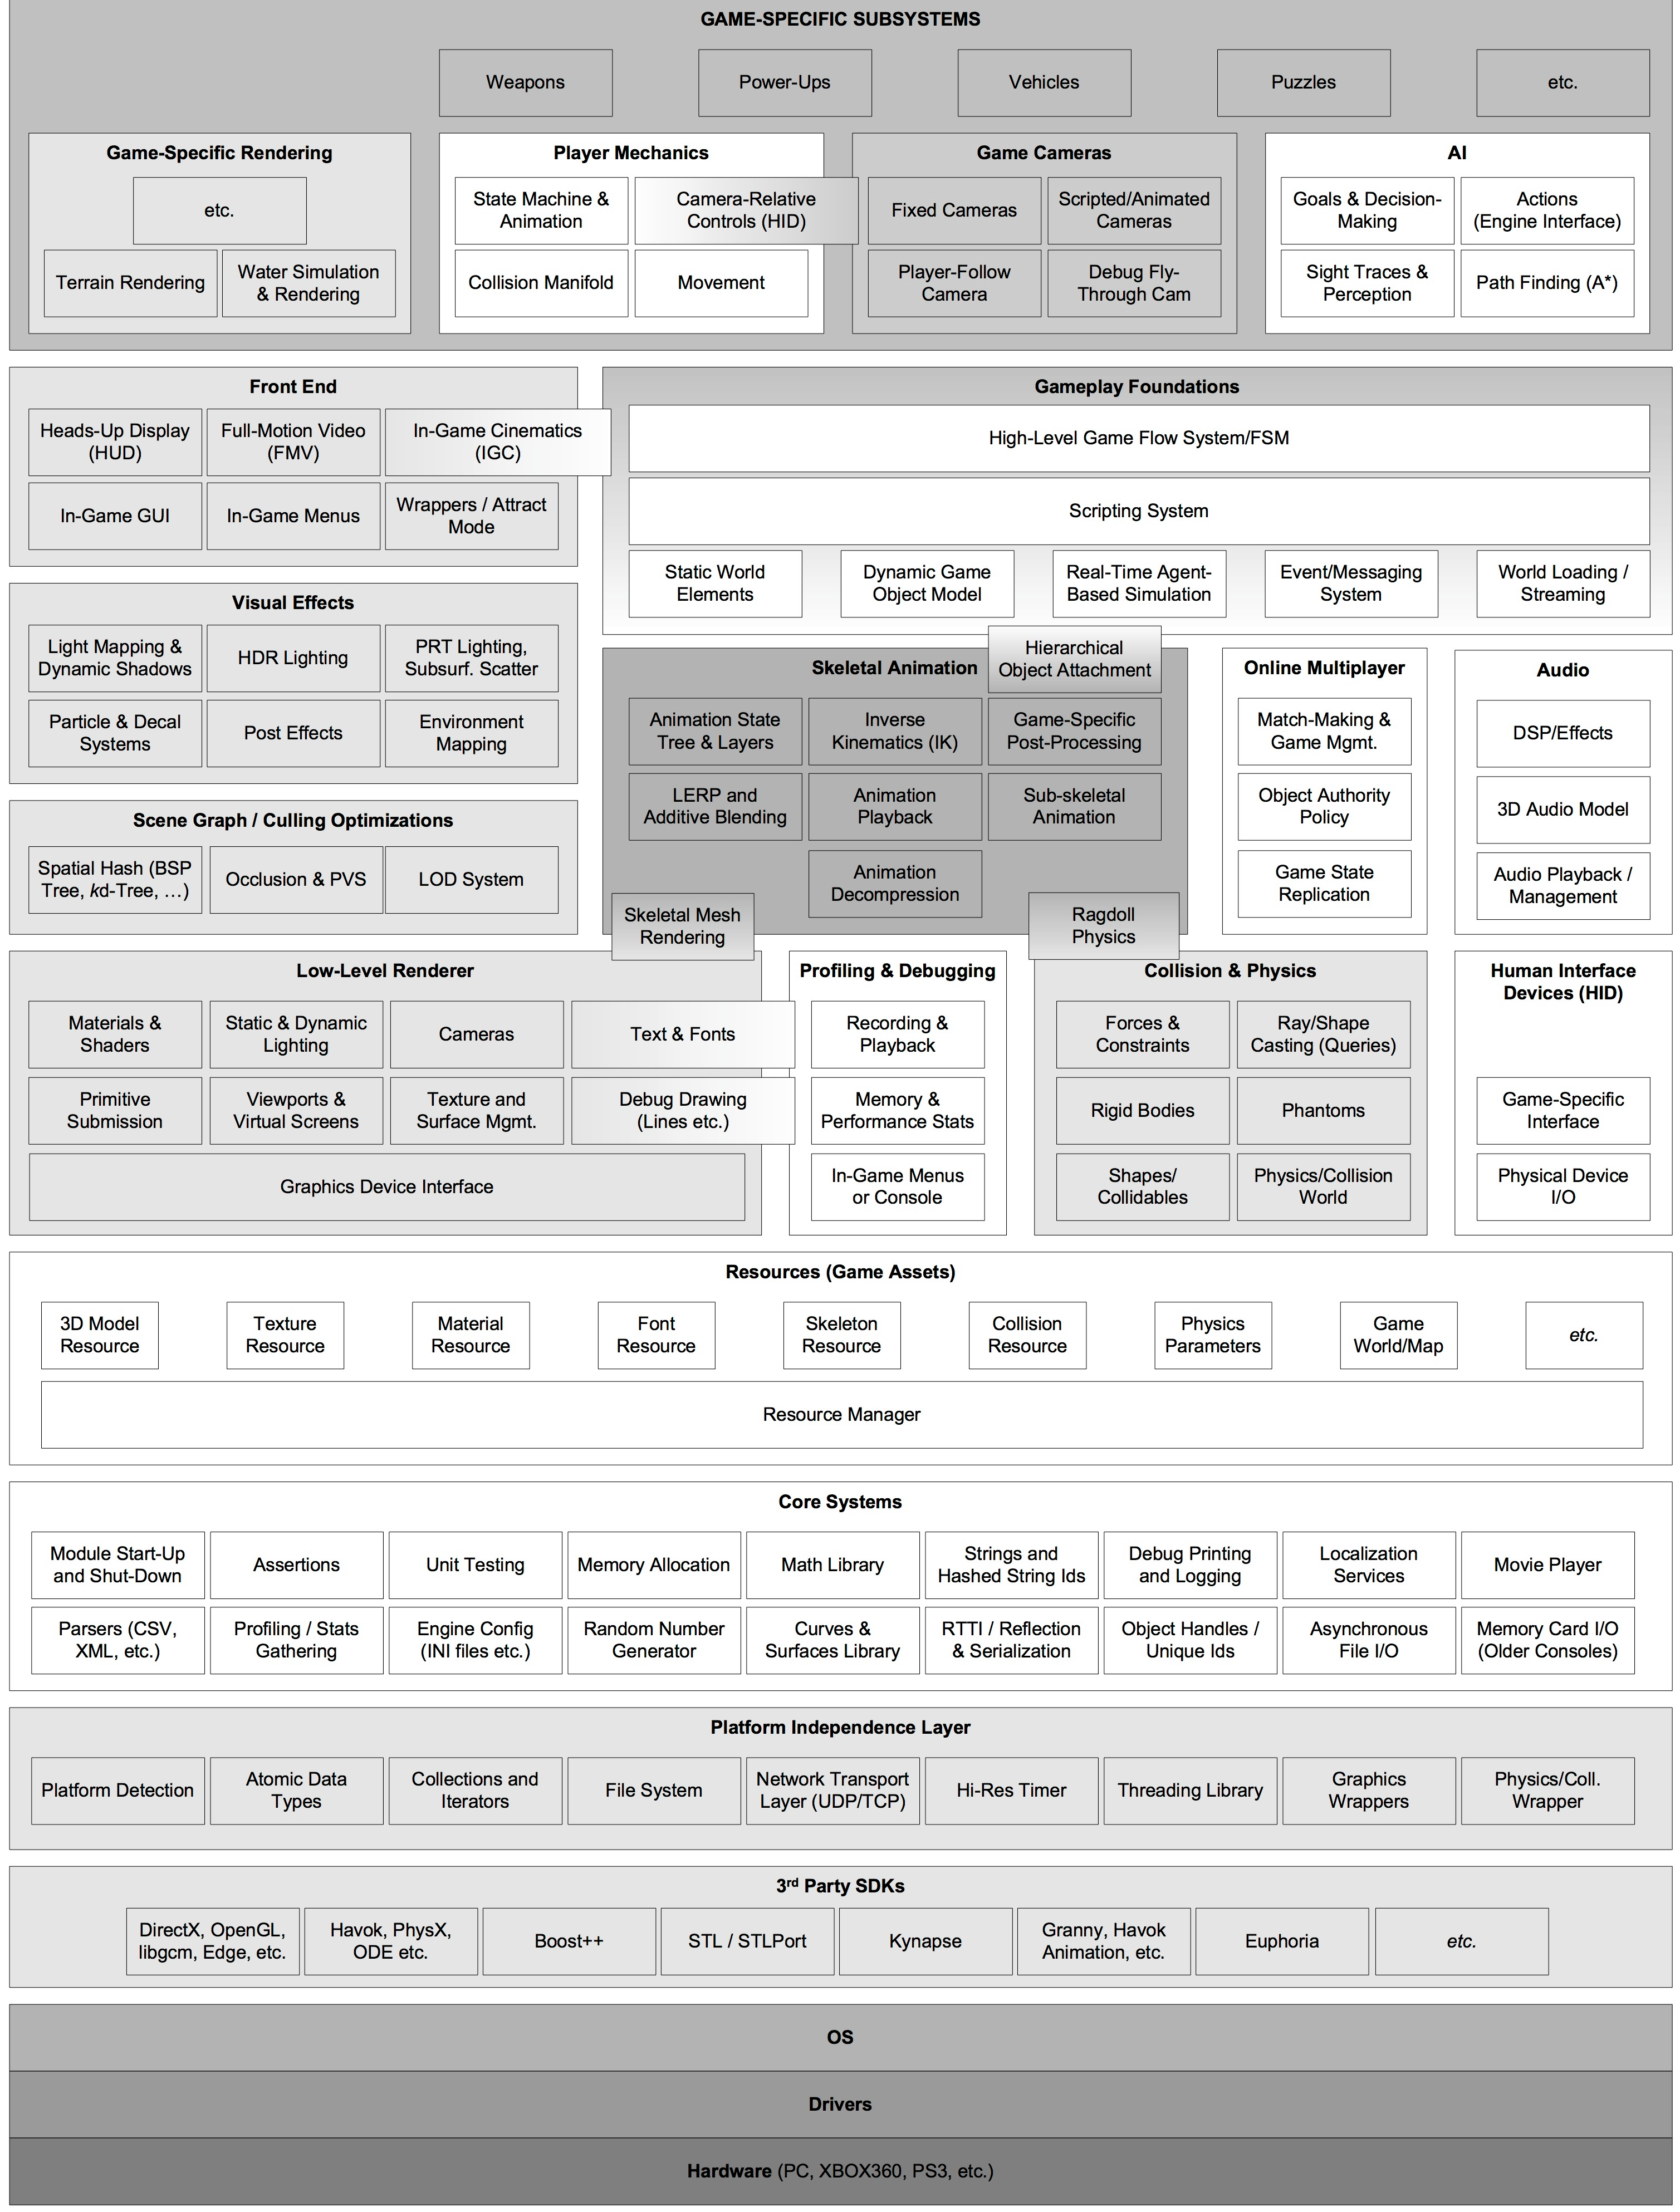
\includegraphics[width=160mm]{Images/game_engine_architecture}
		\caption{Game Engine Architecture}
		\label{fig:Game Engine Architecture}
	\end{figure}	
	
	\chapter{Core}
	
	\chapter{Διαδικτύωση}
		Διαδικτύωση στα ηλεκτρονικά παιχνίδια έχουμε όταν περισσότεροι από ένας παίχτες σε διαφορετικές πλατφόρμες ή υπολογιστές, μοιράζονται και αλληλεπιδρούν στο ίδιο εικονικό περιβάλλον. 
		
		\subsection{Το πρόβλημα}
		\paragraph{Περιγραφή του προβλήματος}
		Διάφοροι παίχτες σε διάφορα σημεία του πλανήτη θέλουν να μοιραστούν ένα εικονικό περιβάλλον σε πραγματικό χρόνο με σκοπό την συνεργασία ή την αντιπαλότητα. O κόσμος είναι ένα υπερσύνολο του offline κόσμου με επιπλέων στοιχεία κοινωνικοποίησης όπως η επικοινωνία μέσω μηνυμάτων ή φωνής.
		
		\paragraph{Κατανόηση του προβλήματος}
		
		Ένας εικονικός κόσμος, περιλαμβάνει πολλές οντότητες οι  οποίες αλληλεπιδρούν μεταξύ τους μέσω των μηχανισμών, νόμων και κανόνων που διέπουν τον κόσμο. Παράδειγμα μηχανισμού είναι η προσομοίωση του φυσικού κόσμου, όπου οι οντότητες αναποκρίνονται σε νόμους της φυσικής.
		
	    Κατά την ενημέρωση του κόσμου, ο προσομοιωτής χρησιμοποιώντας  τους νόμους, τους κανόνες και τους μηχανισμούς που διέπουν τον κόσμο, παίρνει ως είσοδο τις οντότητες, τα ειδικά βάρη των ιδιοτήτων τους, την απόλυτη θέση τους στο σύστημα συντεταγμένων του κόσμου, και το χρονικό διάστημα της προσομοίωσης και αναλύει την προσομοίωση. Η ανάλυση της προσομοίωσης για να είναι επιτρεπτά ακριβής πρέπει να γίνεται περίπου 80-100 φορές το δευτερόλεπτο. [αναφορά σε πηγή]
		
		Στο τέλος της προσομοίωσης, η μηχανή γραφικών αποτυπώνει τον κόσμο στις εξόδους με αναφορές σε στατικά assets, σε αλγόριθμους παραγωγής δυναμικών assets για την αναπαράσταση του κόσμου.
	
		\paragraph{Εξαγωγή απαιτήσεων}	
		Με βάση το πρόβλημα καταλήγουμε στο παρακάτω διάγραμμα ακολουθίας.
		
		\begin{figure}[h]
			\centering
			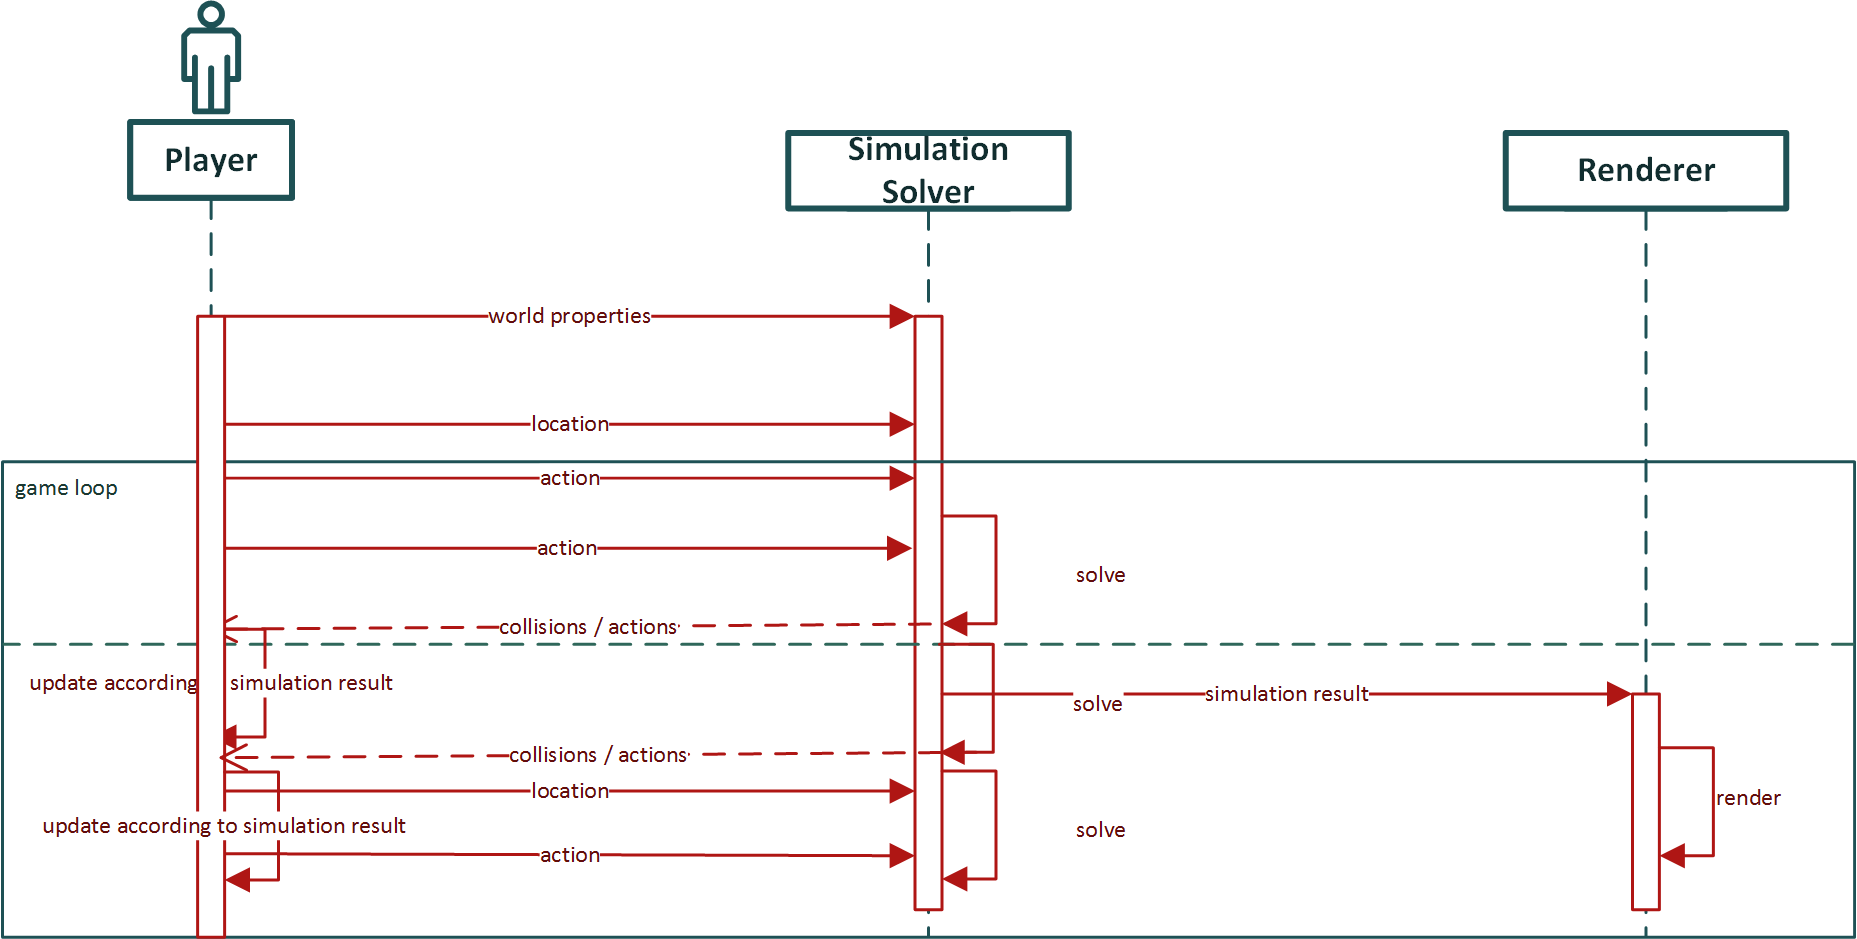
\includegraphics[width=140mm]{Images/gameloop_network_sequence}
			\caption{Network Sequence}
			\label{fig:Network Sequence}
		\end{figure}		
		
		Βλέποντας το διάγραμμα καταλαβαίνουμε ότι σε η διαδικασία rendering περιλαμβάνει στατικά στοιχεία και αλγόριθμους, τα οποίοι μπορούν να φορτώνονται τοπικά στον κάθε υπολογιστή, και δεν είναι απαραίτητα για την επίλυση της προσομοίωσης. Τα απαραίτητα στοιχεία για την προσομοίωση τα οποία πρέπει να μοιράζονται μεταξύ των παιχτών είναι:
		\begin{itemize}
			\item Oι ιδιότητες της οντότητας με βάση τους νόμους του κόσμου. Οι ιδιότητες αυτές δεν ενημερώνονται συχνά.
			\item Οι αλλαγές στο σύστημα συντεταγμένων και οι διάφορες ενέργειες της κατευθυνόμενης οντότητας κατά την πάροδο του χρόνου. Οι αλλαγές τοποθεσίας και ενέργειες γίνονται πολλές φορές ανά δευτερόλεπτο. Η προσομοίωση για να είναι ακριβής πρέπει να ενημερώνεται για τις διάφορες ενέργειες σε πραγματικό χρόνο.
		\end{itemize}
				
		\subsection{Εκπόνηση σχεδίου}	
		Η ανάγκη αποστολής πολλών μηνυμάτων ανά δευτερόλεπτο οδηγεί στη χρήση των network sockets. Τα sockets χρησιμοποιωντας ένα IP και  Port και επιτρέπουν την αποστολή και παραλαβή μηνυμάτων με βάση κάποιου πρωτόκολλου.
		
		\paragraph{Επιλογή πρωτοκόλου}
		\begin{itemize}	
			\item[TCP] Το TCP (transmission control protocol), είναι το πιο συχνά χρησιμοποιημένο πρωτόκολλο. Η διασύνδεση με TCP είναι αξιόπιστη και τα μηνύματα παραλαμβάνονται στη σειρά αποστολής. Η αξιοπιστία όμως έρχεται με ένα μικρό κόστος απόδοσης.
			\item[UDP] Το UDP (user diagram protocol) δεν περιλαμβάνει την αξιοπιστία και την εγγύηση της αλληλουχίας μηνυμάτων. Η απουσία λειτουργιών όμως, το κάνει το πιο γρήγορο σε αποστολή μηνυμάτων πρωτόκολλο.
			
			Η επιλογή πρωτοκόλλου γίνεται ανάλογα με το γενικότερο πλαίσιο και τη συγκεκριμένη χρήση του πακέτου αποστολής. Στην αποστολή της τοποθεσίας, το οποίο γίνεται 20φορές / δευτερόλεπτο, η αξιοπιστία δεν είναι το βασικότερο, αλλά η απόδοση. Στην αποστολή των στοιχειών του χρήστη κατά την έναρξη, ή ενώς γραπτού μηνύματος πρέπει να είναι αξιόπιστη.
		\end{itemize}

		\paragraph{Επιλογή αρχιτεκτονικής δικτύου}
			Οι αρχιτεκτονικές δικτύου χωρίζονται ανάλογα με το που γίνεται η επίλυση και επεξεργασία της προσομοίωσης.  
		\begin{itemize}	
			\item[Client-server model] στο οποίο ο client απλά κάνει render και το μεγαλύτερο κομμάτι της λογικής και της προσωμοίωσης τρέχει στον server. Ο server στέλνει οδηγίες στον client για το τι να κάνει render και ο client απλά υπακούει.
			\item[Client on top of server model] ο client είναι και server, δηλαδή οι μηχανές που έχουν τον client έχουν και τον server.
			\item[Peer-to-peer] οι μηχανές συμπεριφέρονται μερικώς ως clients και μερικώς ως servers, δηλαδή έχουν και στοιχεία λογικής και επεξεργασίας.
		\end{itemize}
			Η client-server αρχιτεκτονική εφαρμόζεται σε παιχνίδια τα οποία περιλαμβάνουν πολύ μεγάλους κόσμους και η προσομοίωση περιλαμβάνει αλληλεπιδράσεις μεταξύ πολλών οντοτήτων. Οι προσωμοιώσεις αυτές γίνονται σε εξειδικευμένες μηχανές και όχι στον προσωπικό υπολογιστή του κάθε χρήστη γιατί χρειάζονται μεγάλους υπολογιστικούς πόρους. Επίσης ο server μπορεί να λύσει race conditions και να λειτουργήσει ως "διαιτητής" μεταξύ δύο οντοτήτων οι οποίες ζητούν πρόσβαση στο ίδιο σύστημα κατά το ίδιο χρονικό διάστημα. Οι αρχιτεκτονικές στις οποίες ο client περιλαμβάνει στοιχεία επεξεργασίας του κοινόχρηστου κόσμου, είναι πιο δύσκολες στην ανάπτυξη συντήρηση γιατί δημιουργούνται race conditions στο χρονικό διάστημα αποστολής-παραλαβής μηνυμάτων που προορίζονται σε αλληλοεξαρτώμενες λειτουργίες.
			
		\subsection{Σχεδίαση του framework}
		Κατά το σχεδιασμό διαδικτυακών παιχνιδιών πολλά μοτίβα και στερεότυπα κώδικα επαναλαμβάνονται χωρίς να συμβάλλουν στην λογική ή μηχανισμούς. Σκοπός του framework είναι να μειώσει και να απλοποιήσει τον επαναλαμβανόμενο κώδικα και να προμηθεύσει τον χρήστη με μοτίβα και μοντέλα ούτως ώστε να εστιάσει μόνο στα απαραίτητα.
		
		\subsection{Έννοιες}
		\paragraph{Serialization}
		Σε μια αντικειμενοστραφή γλώσσα χρησιμοποιούνται κλάσεις για να μοντελοποιήσουν το πρόβλημα. Όμως τα αντικείμενα τον κλάσεων δεν μπορούν να σταλούν μέσω network socket στην αρχική τους μορφή, πρέπει να γίνει μια μετατροπή σε binary για να είναι συνεπής με το format των δεδομένων που αποστέλλονται μέσω του socket . Κατά την αποστολή έχουμε το serialization τον αντικείμενων, και κατά την παραλαβή το deserialization του πακέτου στο αντικείμενο που αντιπροσωπεύει.
		\paragraph{Message Types}
		Οι διάφοροι τύποι μηνυμάτων χρησιμοποιούνται για να ξεχωρίσουν την κατάσταση στην οποία βρίσκεται ο client ή ο server.
			\begin{itemize}
				\item[Αλλαγή κατάστασης] info
				\begin{itemize}
					\item [Connecting] info
					\item [Connected] info
					\item [Disconnecting] info
					\item [Disconnected] info
				\end{itemize}
				\item [Data] info
				\item [ErrorMessage] info
				\item [WarningMessage]
				\item [VerboseMessage]
				\item [ConnectionApproval]
				\item [DiscoveryRequest]
				\item [DiscoveryResponse]
			\end{itemize}
		Οι τύποι μηνυμάτων μπορούν να μοντελοποιηθούν ως ένα enum και να προστεθεί η πληροφορία τους στο πρώτο byte του serialized μηνύματος. Το πρώτο byte του παραληφθέντα μηνύματος περιλαμβάνει τον τύπο του μηνύματος.
		
		\paragraph{NetworkManager}
		Ο network manager είναι υπεύθυνος για την διαχείριση των sockets, την αποστολή / παραλαβή μηνυμάτων, ενθυλακώνει λειτουργιες για την διαδικτύωση και είναι ο πηρύνας του framework και επεκτίνεται από τον client, server οι οποίοι προσθέτουν λειτουργίες.
			
		\subsection{Υλοποίηση}	
		\paragraph{Τρόπος χρήσης}
		Η διαδικασία χρήσης πρέπει να είναι εξορθολογιστική και ξεκάθαρη για εύκολη και γρήγορη ανάπτυξη και περιοριστική για αποφυγή bugs και προβληματων.
		\begin{figure}
			\centering
			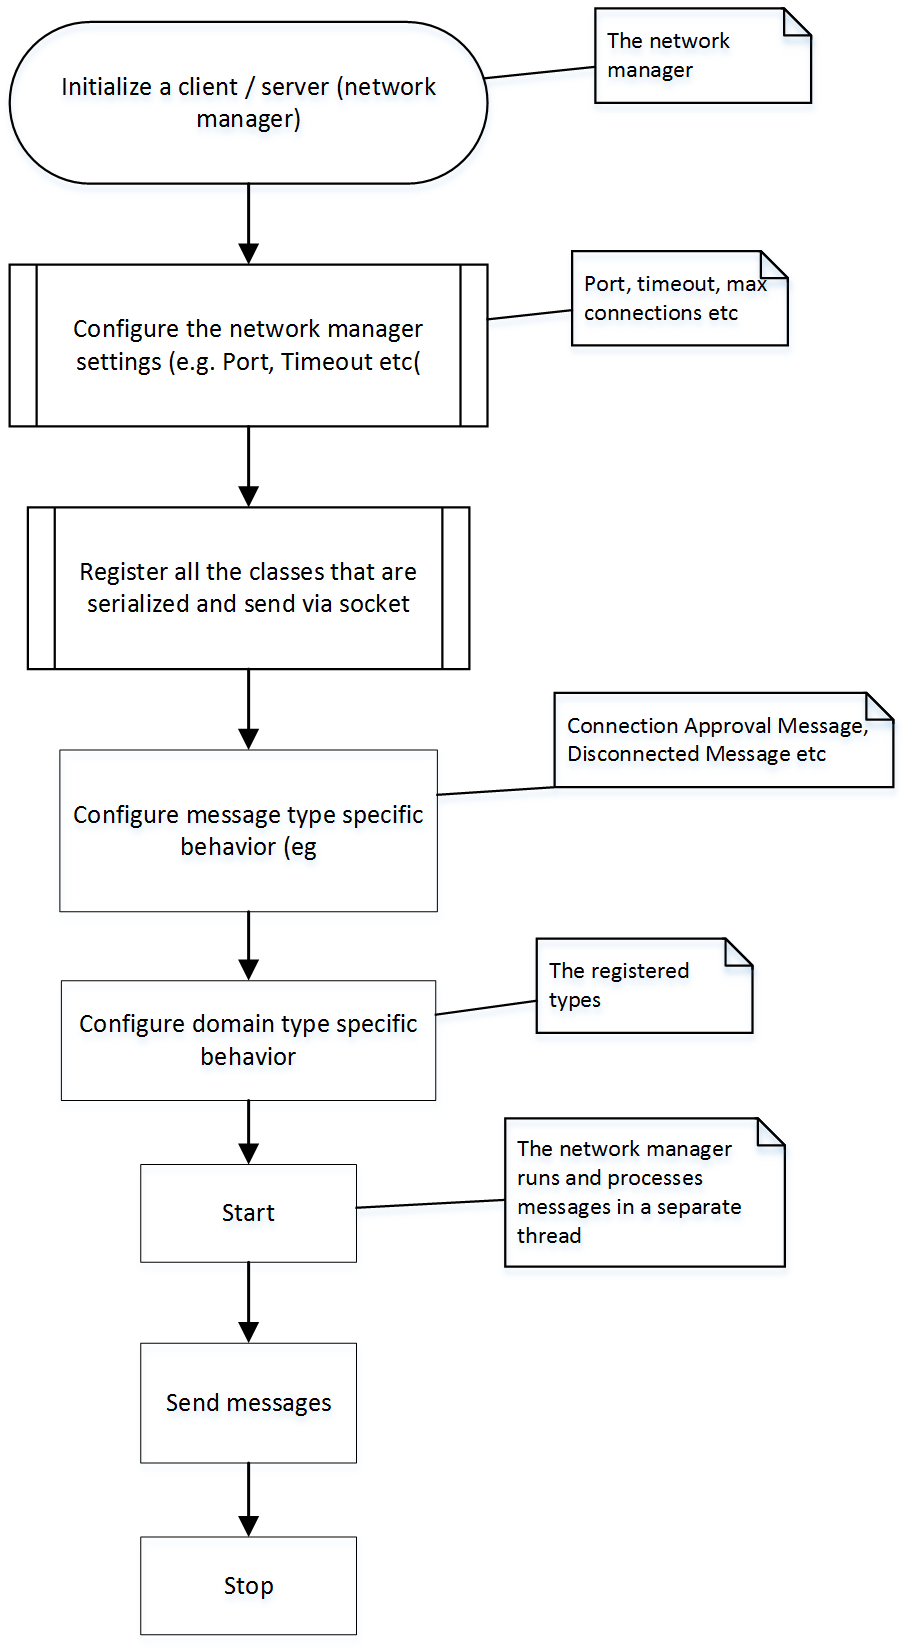
\includegraphics[width=100mm]{Images/network_usage_diagram}
			\caption{Network Usage Diagram}
			\label{fig:Network Usage_Diagram}
		\end{figure}	
					
		\subsection{Αρχιτεκτονική}	
		Η αρχιτεκτονική στηρίζεται στην ανταλλαγή μηνυμάτων-κλάσεων και χωρίζεται στα παρακάτω επίπεδα.
			\begin{itemize}
				\item {Packages} Χειρίζεται το serialization, αναλύει τα εισερχόμενα μηνύματα και χειρίζεται τις ανακατευθύνσεις του εκτελούμενου κώδικα κατά την παραλαβή μηνυμάτων. 
				\item {Networking} Διαχειρίζεται τις συνδεσεις των χρηστών, τα sockets και ο,τι έχει να κάνει με διασύνδεση.
				\item {Auditing} Αφαιρετικό επίπεδο για logging. Ο χρήστης μπορεί να ενσωματώσει τη δική του λογική παρακολούθησης μηνυμάτων.
				\item{Infrastructure} Το επίπεδο αυτό περιέχει επαναχρησιμοποιήσημο κώδικα των πακέτων όπως το ConcurrentRepository, για thread-safe αποθήκευση κλειδιών και τιμών, και το ParallelBufferBlock το οποίο εκτελεί κώδικα σε buffer άλλου thread για ασύγχρονη επεξεργασία.
			\end{itemize}
			
			\paragraph{Packages Module}	 
			Το serialization των μηνυμάτων πρέπει να είναι ντερερμενιστικό ώστε να αναγνωρίζεται ο τύπος του μηνύματος και η κλάση την οποία αντιπροσωπεύει και ελαφρύς ώστε να μην επιβαρύνεται το network με επιπλέον δεδομένα. Ο ενσωματομένος serializer χρησιμοποιεί reflection για να αναγνωρίσει τα primitive properties της κλάσης. Για προχωριμένο serialization περίπλοκων τύπων, ο χρήστης έχει τη δυνατότητα να συμπεριλάβει τον δικό του serializer με το implementation του IPackageSerializer interface και την χωρήγηση του σημειώνοντας την κλάση με το PackageSerializerAttribute και τον τύπο του serializer.
			
			
			Κατά την προετοιμασία του network manager, o χρήστης καλείται να καταχωρίσει στο Container ποιες κλασεις θα χρησιμοποιηθούν κατά την ανταλλαγή μηνυμάτων. Οι κλάσεις που προωρίζονται για serialization σημειώνονται με κάποιο Attribute και η καταχώριση μπορεί να γίνει δυναμικά με reflection.
			Όταν τελειώσει η καταχώριση, το container χρησιμοποιώντας ένα ντετερμενιστικό αλγόριθμο ταξινομώντας με βάση το όνομα της κλάσης στο χώρο ονομάτων κτίζει ένα thread safe repository στο οποίο καταχωρείται ένα μοναδικό byte για αναγνωριστικό του κάθε τύπου και πληροφορίες για την χρήση του τύπου.
			
			Στο τέλος της καταχώρισης και της κατασκευής αλγόριθμου αντιστοίχισης αντικειμένων και λογικής, ο χρήστης μπορεί να καταχωρίσει εκτελέσημο κώδικα υπό μορφή function o οποίος εκτελείται ασύγχρονα κατά την παραλαβή κάποιου μηνύματος-κλάσης, τύπου μηνύματος, ή συμβάντος συγκεκριμένης σύνδεσης.
			
			\begin{figure}
				\centering
				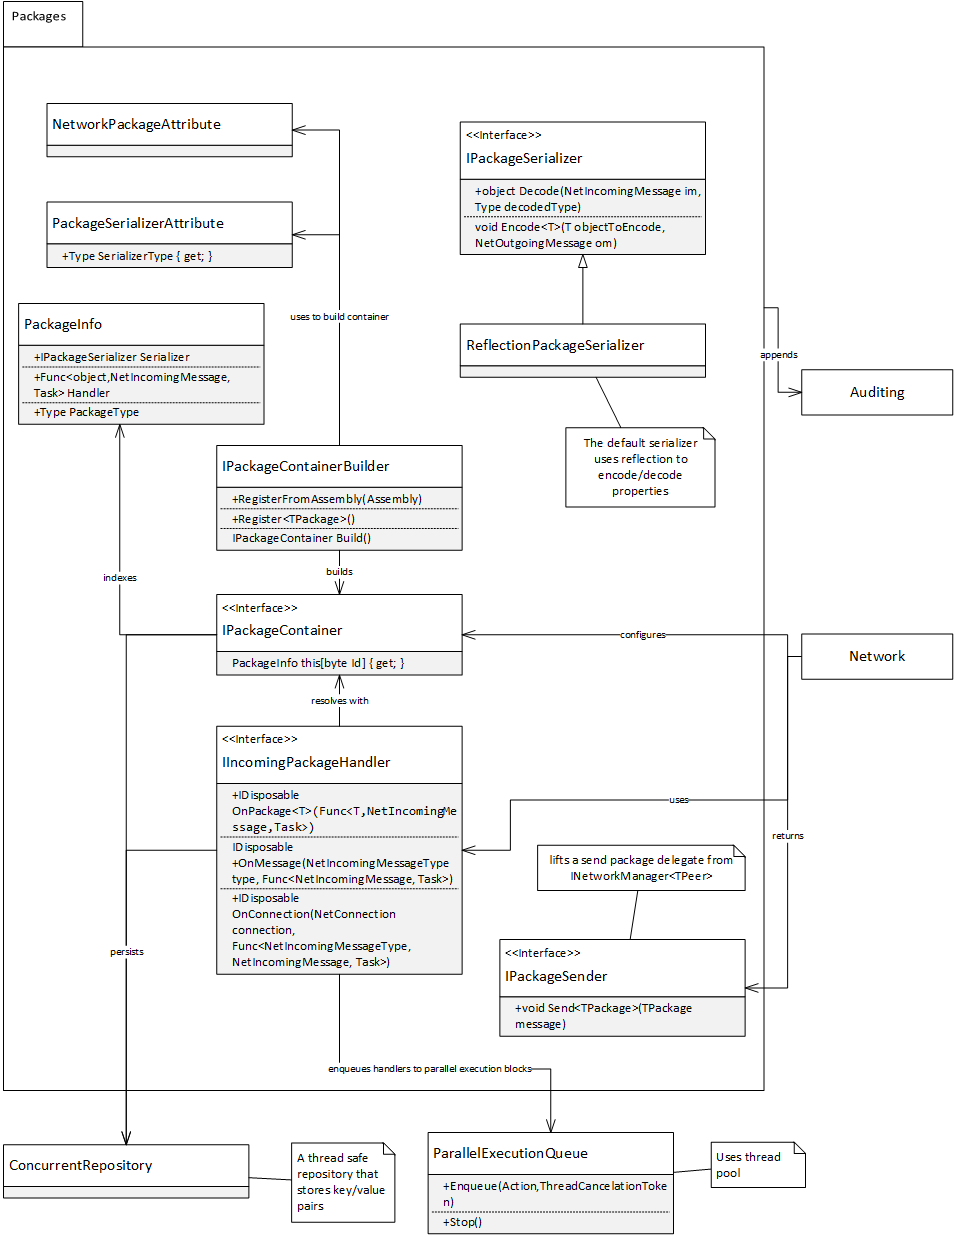
\includegraphics[width=165mm]{Images/network_architecture_packages}
				\caption{Network Packages Module}
				\label{network_packages}
			\end{figure}	
					
			\paragraph{Networking Module}	 					
			
			Οι ρυθμίσεις του network manager κτίζονται από αφαιρέσεις. Η χρήση πρωτοκόλλων και τεχνικών γίνεται με άγνοια της υλοποίησης και λεπτομερειών.
			Η σχεδίαση επιτρέπει την αποστολή μηνύματος ανεξαρτήτου πρωτοκόλου, τρόπο αποστολής και παραλήπτη. Ο network manager περιλαμβάνει τεχνικές function lifting για αποστολή μηνυμάτων. Ο χρήστης μπορεί να ρυθμίσει διάφορους τρόπους αποστολής ανάλογα με το περιβάλλον χρήση, και να τους κρύψει πίσω από functions. 
						
			\begin{figure}
				\centering
				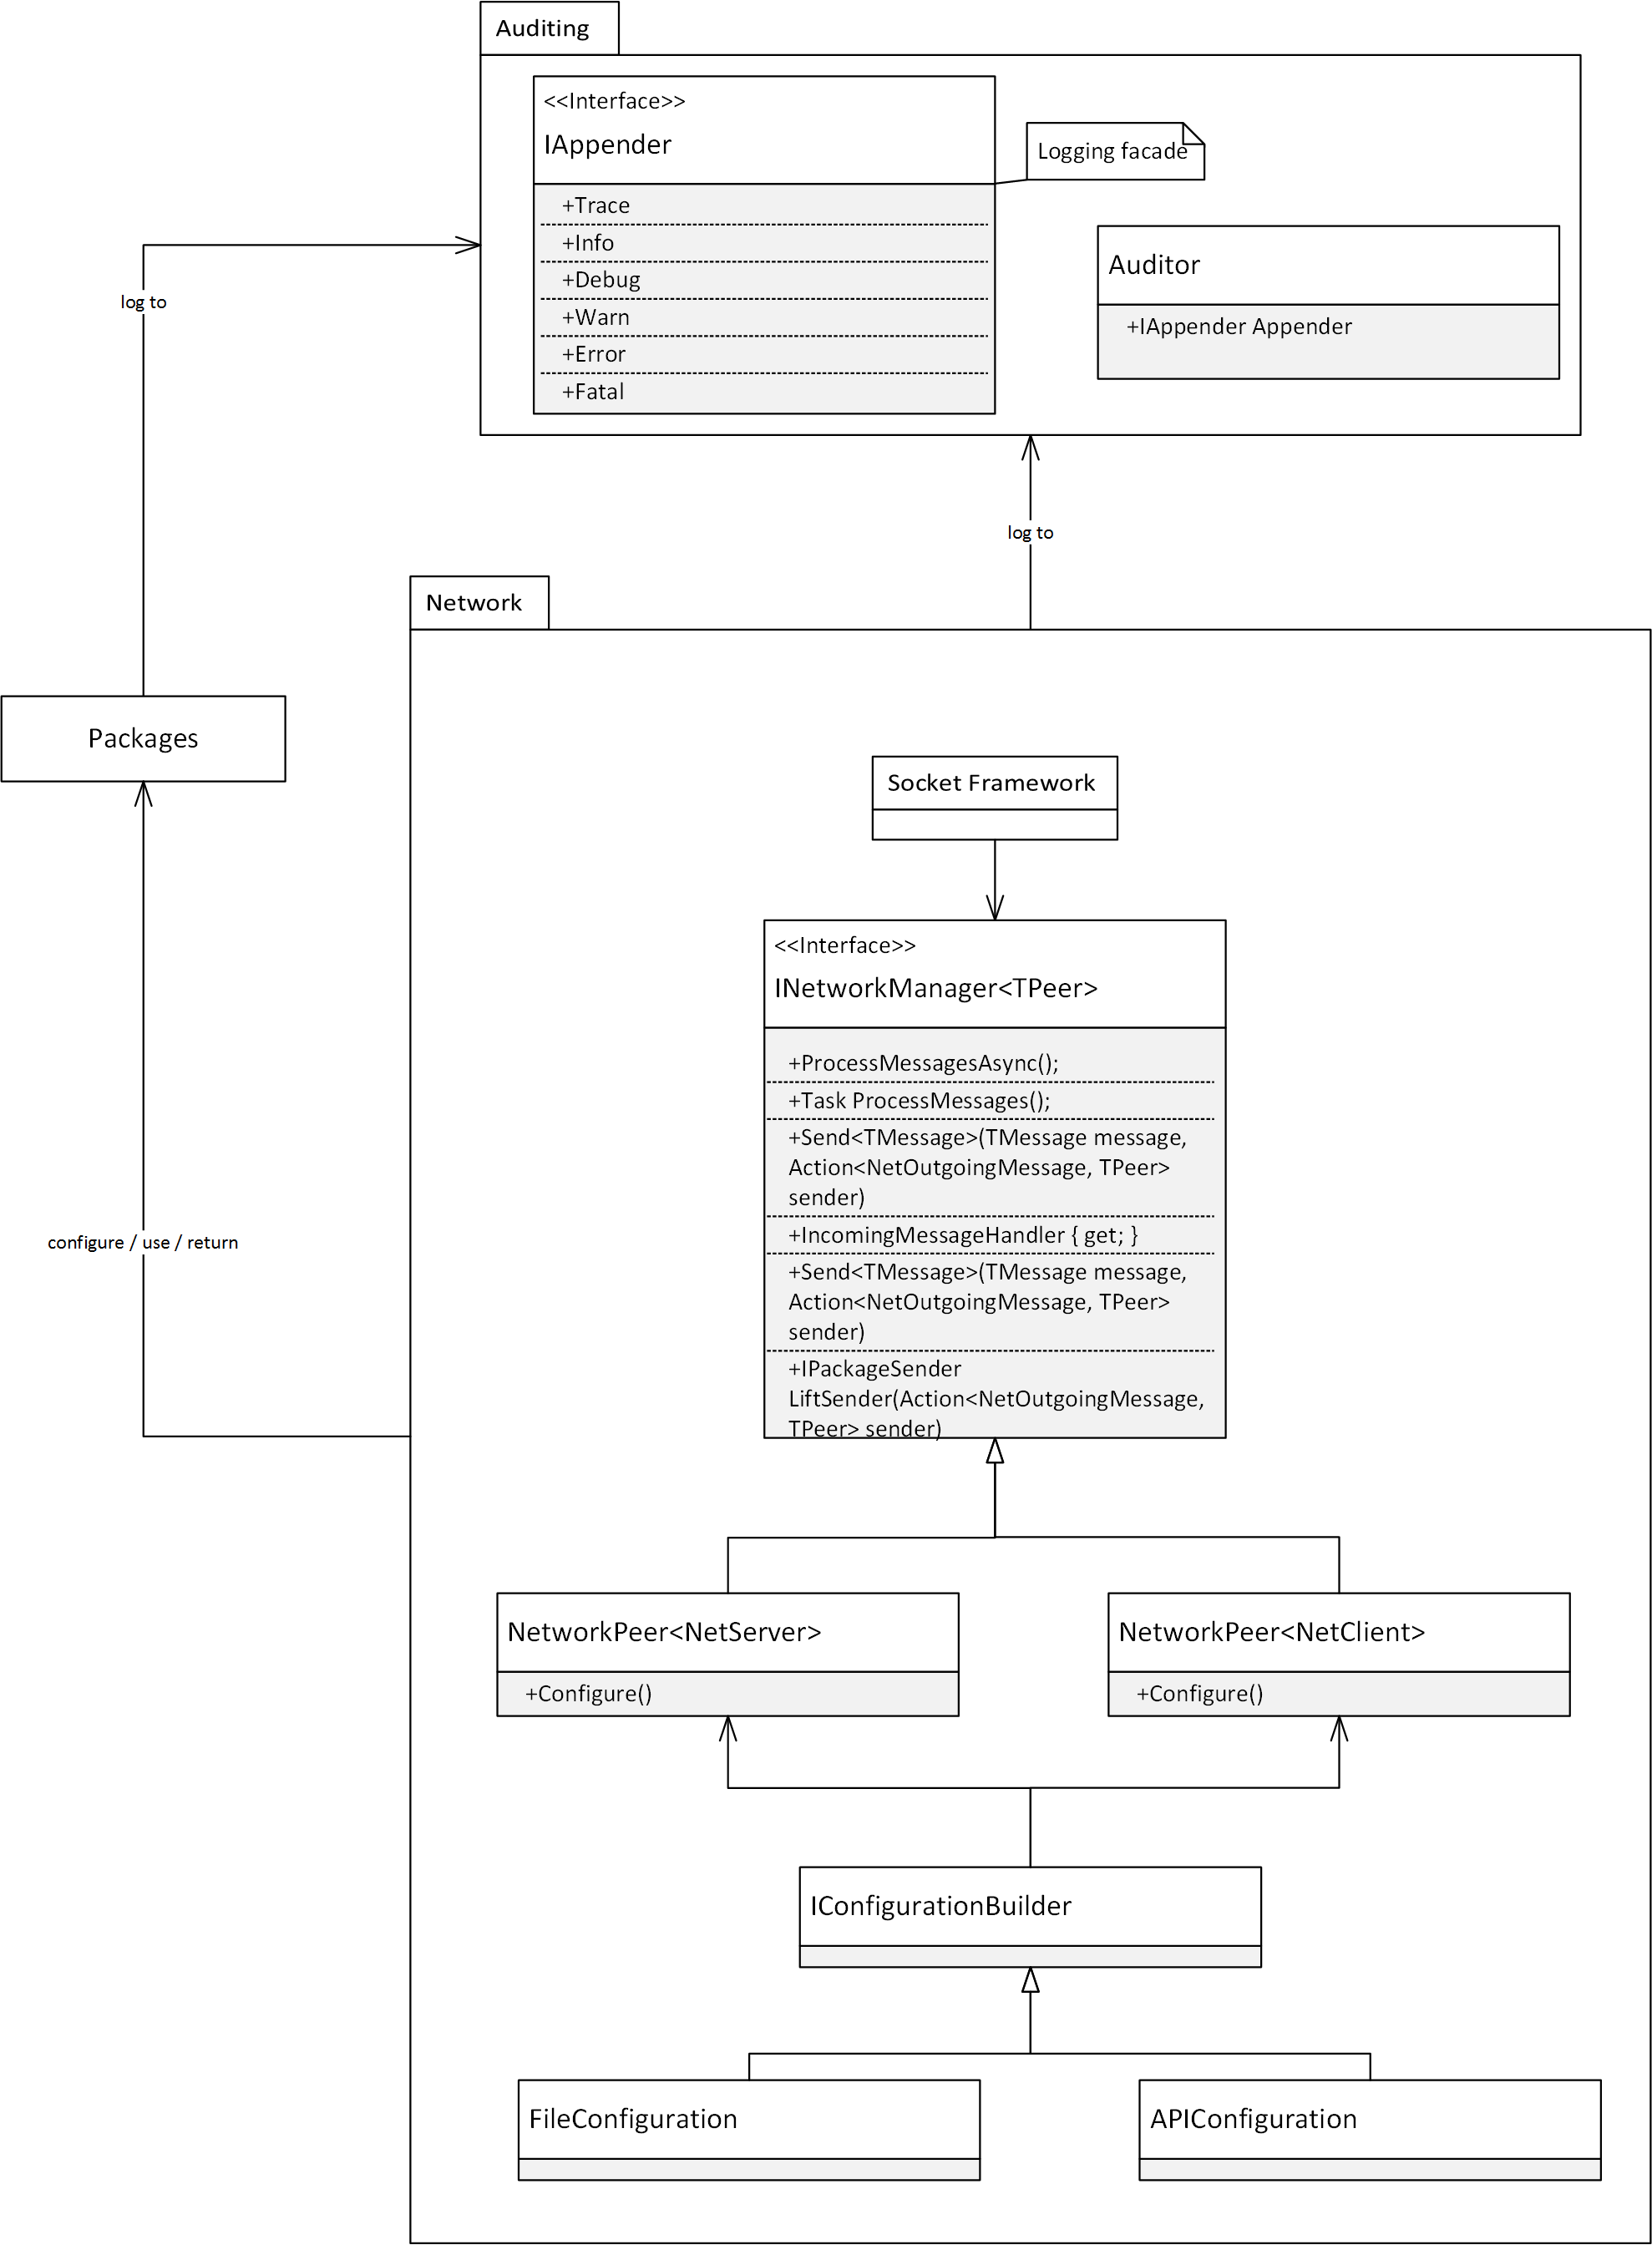
\includegraphics[width=165mm]{Images/network_architecture_networking}
				\caption{Networking Module}
				\label{networking_module}
			\end{figure}		

	\paragraph{API}
	Συντομη επισκόπηση του API.
	\begin{itemize}
		\item Κλάσεις που προορίζονται για ανταλλαγή μηνυμάτων
		\lstset{style=sharpc}
		\begin{lstlisting}
[GinetPackage]
[PackageSerializer(typeof(MyCustomSerializer))] //optional
public class MyPackage
{
    public string Message { get; set; }
}          
		\end{lstlisting}
		\item Ρύθμιση server
		\lstset{style=sharpc}
		\begin{lstlisting}     
var server = new NetworkServer("MyServer",
	builder =>
	{
		//via reflection
		builder.RegisterPackages(Assembly.Load("Packages.Assembly.Name"));
	    //or manually
		builder.RegisterPackage<MyPackage>();
	}
	cfg =>
	{
		cfg.Port = 1234;
		cfg.ConnectionTimeout = 5.0f;
		//Additional configuration
	}
	out: new ActionAppender(Console.WriteLine) //optional, logging output, default is the one supplied			 
		\end{lstlisting}
		\item Καταγραφή κινήσεων		
		\lstset{style=sharpc}
		\begin{lstlisting}
server.IncomingMessageHandler.LogTraffic();
		\end{lstlisting}		
		\item Απάντηση κατά την παραλαβή μηνύματος
		\lstset{style=sharpc}
		\begin{lstlisting}
server.Broadcast<ChatMessage>((msg, im, om) =>
{
	server.Out.Info($"Received {msg.Message}");
	server.SendToAllExcept(om, im.SenderConnection, NetDeliveryMethod.ReliableOrdered, channel: 0);
}, 
packageTransformer: msg => 
msg.Message += "this is broadcasted");	


server.BroadcastExceptSender<ChatMessage>((sender, msg) =>
{
	server.Out.Info($"Broadcasting {msg.Message}. Received from: {sender}");
});
		\end{lstlisting} 		

		\item Κώδικας ο οποίος εκτελείται κατά την παραλαβή συγκεκριμένου τύπου μηνύματος
		\lstset{style=sharpc}
		\begin{lstlisting}
server.IncomingMessageHandler.OnMessage(NetIncomingMessageType.ConnectionApproval, incomingMsg =>
{
	//Configure connection approval
	var parsedMsg = server.ReadAs<ConnectionApprovalMessage>(incomingMsg);
	if(parsedMsg.Password == "my secret and encrypted password")
	{
		incomingMsg.SenderConnection.Approve();
		incomingMsg.SenderConnection.Tag = parsedMsg.Sender;
	}
	else
	{
		incomingMsg.SenderConnection.Deny();
	}
});
		\end{lstlisting}
		\item Εκτελέσιμος κώδικας κατά την παραλαβή συγκεκριμένου μηνύματος-κλάσης
		\lstset{style=sharpc}
		\begin{lstlisting}
server.IncomingMessageHandler
.OnPackage<MyPackage>((msg, sender) => 
	Console.WriteLine($"Received {msg.Message} from {sender.SenderConnection}"));
		\end{lstlisting}	
		\item Αποστολή μηνύματος-κλάσης
		\lstset{style=sharpc}
		\begin{lstlisting}
server.Send(new MyPackage { Message = "Hello" },
	(outgoingMessage,peer) => 
		peer.SendMessage(outgoingMessage,NetDeliveryMethod.ReliableOrdered));
		\end{lstlisting}		
		\item Lift αποστολής μηνύματος
		\lstset{style=sharpc}
		\begin{lstlisting}
		var packageSender = client.LiftSender((msg, peer) =>
		peer.SendMessage(msg, NetDeliveryMethod.ReliableOrdered));
		
		packageSender.Send(new MyPackage { Message = "Hello" });	
		\end{lstlisting}	
		\item Διαγραφή handler
		\lstset{style=sharpc}
		\begin{lstlisting}	
		var handlerDisposable = server.IncomingMessageHandler
		.OnPackage<MyPackage>((msg, sender) => {}));
		
		handlerDisposable.Dispose();	
		\end{lstlisting}		
		\item Η ρύθμιση και το API του client είναι πανομοιότυπo με του server. Στη θέση του \textit{NetworkServer} χρησιμοποιείται ο \textit{NetworkClient} όπου και τα δύο υλοποιούν τον \textit{NetworkManager<TPeer> where TPeer:NetPeer}		
	\end{itemize}
	
	\subsection{Testing}
	Μια καλή αρχιτεκονική υποστηρίζεται από την ευκολία της δοκιμαστικότητας ανά μονάδα (unit testability). Το framework χρησιμοποιεί functional τεχνικές, οι οποίες εύκολα μπορούν να αντικατασταθούν με mocks. Ο χρήστης μπορεί να απομιμήσει την παραλαβή ή αποστολή πακέτων και να ενημερώνει την μονάδα επεξεργασίας μηνυμάτων από το τρέχων thread.
	
	\lstset{style=sharpc}
	\begin{lstlisting}
	
[TestMethod]
public void Incoming_Package_GetsHandled()
{
	//Arrange
	var client = new NetworkCliient(
		builder => 
			builder.Register<MyPackage>(),
		cfg=> {});
		
	var mockedHandler = new MockFunc<MyPackage,NetIncomingMessage>();
	mockedHandler.Setup( x => 
		x(It.IsAny<MyPackage>()));
	
	client
	.IncomingMessageHandler
	.OnPackage<MyPackage>(mockedHandler);	
	
	//Act	
	client.IncomingMessageHandler.SimulateReceive(new MyPackage());	
	client.ProcessMessages().RunSynchronously();
	
	//Assert
	mockedHandler.Verify(x=>x(), Times.Once()));
}
	\end{lstlisting}
		
	Επίσης παρέχεται η δυνατότητα της προσομοίωσης χαμένων πακέτων, για να δοκιμαστεί πως η εφαρμογή ανταποκρίνεται σε περιβαλλον κακής διαδικτύωσης και να αναπτυχθούν τεχνικές network prediction για εξομάλυνση της κίνησης.
	
	
	\subsection{Ανάλυση των επιδόσεων}
	Benchmarkings table here
	
	\subsection{Επεκτασιμότητα}
	Lobbies and matchmakings
	
	

	\section{Αρχιτεκτονική}		
	
	\chapter{Περίληψη}
	
	\begin{Glossary}
		Το γλωσσάρι μπορεί να είναι χρήσιμο αν χρησιμοποιείτε πολλά ακρώνυμα
		και συντομογραφίες. Για παράδειγμα
		\begin{description}
			\item[TCP]Transmission Control Protocol
		\end{description}
	\end{Glossary}
	
	\printbibliography
	%\lastpageinfo
	

\end{document}
